\documentclass[aspectratio=1610]{beamer}
\usepackage{style}
\graphicspath{{./assets/images}}

\title{Studiare Informatica}
\author{Filippo Daniotti}
\date{6 Febbraio 2021}
\logo{
\includegraphics[height=0.8cm]{logo-small.jpg}}
\institute[DISI]{Dipartimento di Ingegneria e Scienza dell'Informazione}

\AtBeginSection[] {
  \begin{frame}{Indice}
    \tableofcontents[currentsection]
  \end{frame}
}

% arara: pdflatex: { shell: yes, synctex: yes }
% arara: latexmk: { clean: partial }
\begin{document}
	\begin{frame}[plain]
		\addtocounter{framenumber}{-1}
		\centering
		
\includegraphics[width=0.5\textwidth, keepaspectratio]{logo-unitn.eps}		
		\titlepage
	\end{frame}

	% \begin{frame}{Table of Contents}
	% 	\tableofcontents
	% \end{frame}

	\section{Introduzione e contesto}
	\begin{frame}[fragile]{Che cos'è l'informatica?}
		\pause
		\begin{center}
			\Large{TL;DR}\\
		\end{center}		
		È tante cose, dare una definizione precisa ad alta voce lascia interdetto qualsiasi interlocutore. In un certo senso è quasi più utile parlare di cosa \alert<1>{non} è, questo se non altro ci aiuta a non fare assunzioni sbagliate.\\
		\bigskip
		\pause
		Giusto per puntualizzare quelle che sono di certo ovvietà, l'informatica \emph{non} è:
		\begin{columns}
			\begin{column}{0.55\textwidth}
				\begin{itemize}
					\item l'ECDL 
					\item hackerare i profili social 
					\item preparare le crack per i videogiochi 
					\item riparare i computer \Large{AHHHHHHHH} 
				\end{itemize}		
			\end{column}
			\onslide<3-> {
				\begin{column}{0.4\textwidth}
					% inserire memino qui sul riparare i computer + esprienza 150h
					\begin{figure}
						
\includegraphics[width=0.5\textwidth, keepaspectratio]{memino.jpg}	
					\end{figure}
				\end{column}
			}
		\end{columns}
	\end{frame}

	\begin{frame}{Daiiii almeno qualcosina per avere un'idea}
		% Secondo Wikipedia:
		% \begin{quote}
		% 	L'informatica è la scienza che si occupa del trattamento dell'informazione mediante procedure automatizzate[...]
		% \end{quote}
		\begin{center}
			\begin{minipage}{\textwidth}
				\begin{block}{Secondo Wikipedia}
					\begin{quote}
						L'informatica è la scienza che si occupa del trattamento dell'informazione mediante procedure automatizzate[...]
					\end{quote}
				\end{block}
			\end{minipage}
		\end{center}
		\vfill
		\onslide<2->{
			Lista assolutamente non esaustiva di ambiti e branche dell'informatica
			\begin{itemize}
				\item Algoritmi e strutture dati
				\item Teoria della calcolabilità/complessità/grafi/automi
				\item Reti di calcolatori
				\item Crittografia e sicurezza
				\item Intelligenza artificiale
				\item Ambiti interdisciplinari: bioinformatica, calcolo quantistico, et cetera
			\end{itemize}
		}
	\end{frame}

	\begin{frame}{Super citazione della vita}
		\only<1-3>{
			\begin{center}
				\begin{minipage}{\textwidth}
					\begin{alertblock}{Attenzione}
						Citazione super boomer con immagine a bassa risoluzione e buono kaffè in omaggio in arrivo fra
					\end{alertblock}	
				\end{minipage}
			\end{center}
		}
		\vfill
		\only<1>{\centering\Huge 3...}
		\only<2>{\centering\Huge 2...}
		\only<3>{\centering\Huge 1...}
		\only<4>{
			\begin{figure}
				\centering
				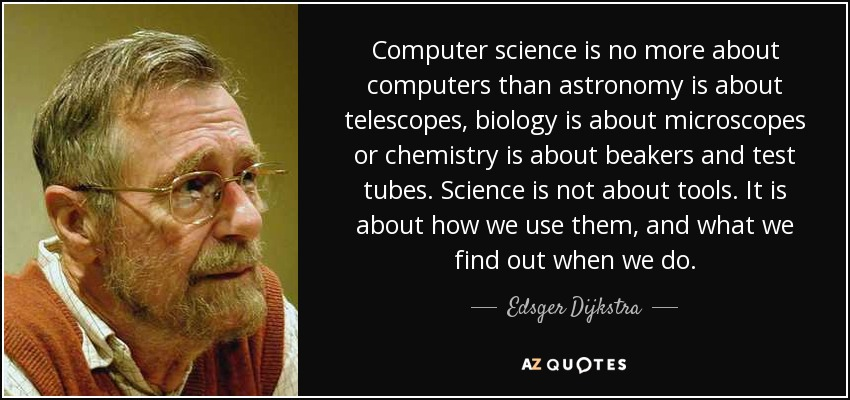
\includegraphics[width=\textwidth, keepaspectratio]{dijkstra.jpg}
			\end{figure}
		}
		\only<5->{
			\begin{figure}
				\centering
				
\includegraphics[width=\textwidth, keepaspectratio]{dijkstra-fragment.jpg}
			\end{figure}
			\visible<6>{
			\begin{center}
				\begin{minipage}{\textwidth}
					\begin{block}{Notate quel \emph{Science}}
						Informatica è a tutti gli effetti una laurea \emph{scientifica}
						\begin{center}
							\begin{tabular}{ c c c }
								Laurea in Informatica & \(\to\) & Scienziato \\
								Laurea in Ingegneria Informatica & \(\to\) & Ingegnere
							\end{tabular}
						\end{center}
					\end{block}
				\end{minipage}
			\end{center}
		}
		}
	\end{frame}

	\section{Cosa si studia}
	\begin{frame}{Sguardo veloce al programma}
		\only<1-2>{
			Io qui mostrerò il programma del Corso di Laurea proposto dall'Università di Trento.\\
			\small{\url{https://offertaformativa.unitn.it/it/l/informatica/regolamenti-e-manifesti}}
		}
		\vfill
		\visible<2>{
			Fate \emph{sempre} riferimento al sito dell'Università che vi interessa.
		}
		\only<3>{
			\centering
			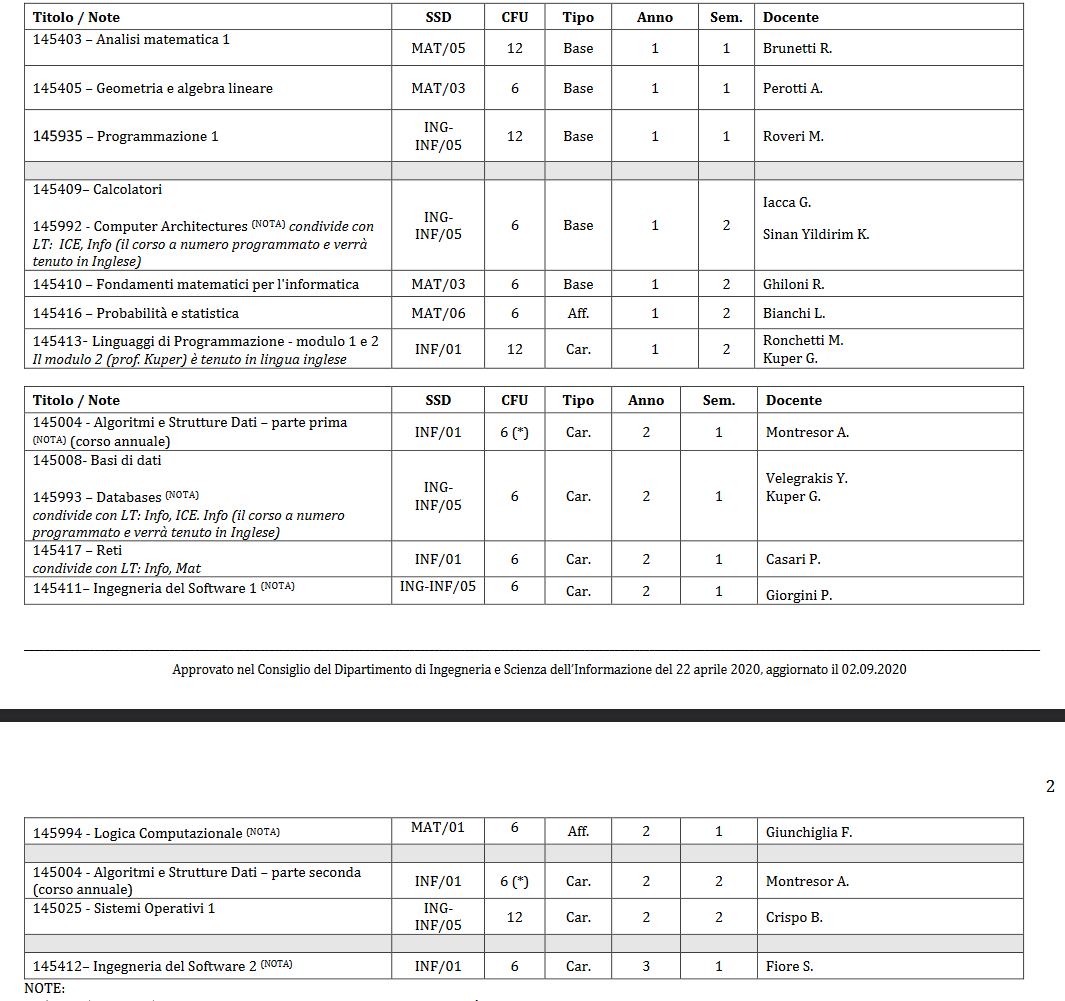
\includegraphics[width=0.6\textwidth, keepaspectratio]{corsi-1.png}
		}
		\only<4>{
			\centering
			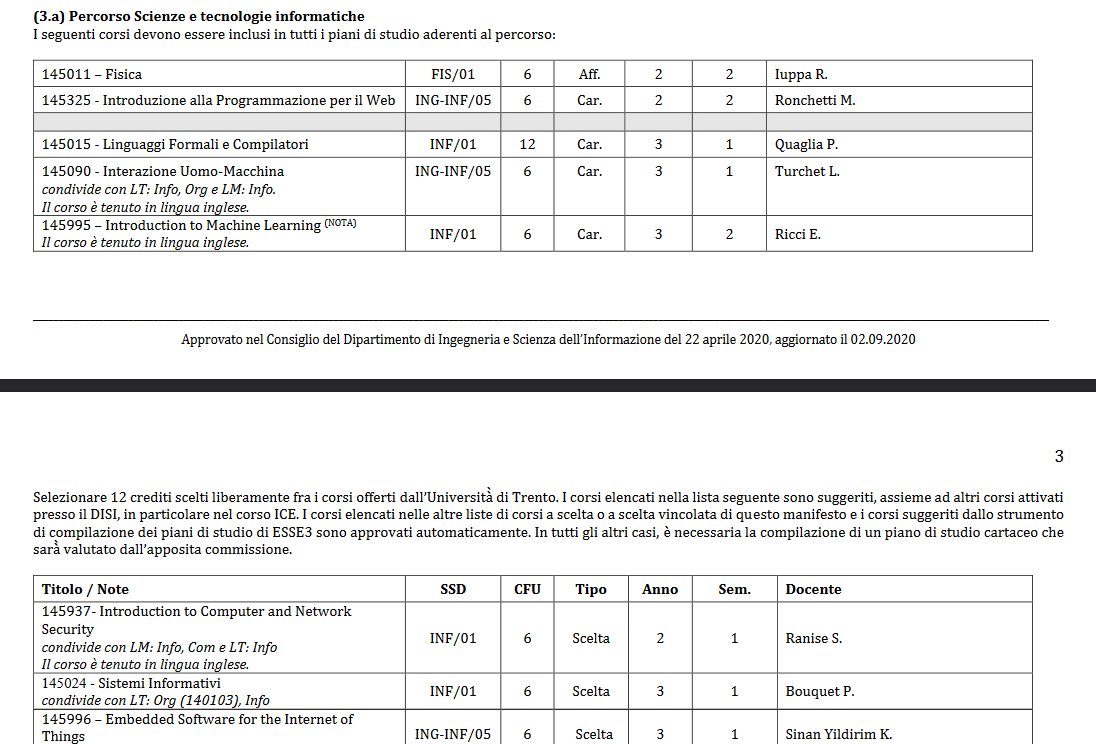
\includegraphics[width=0.8\textwidth, keepaspectratio]{corsi-2.png}
		}
		\only<5->{
			\begin{columns}
				\begin{column}{0.4\textwidth}
					\begin{figure}
						\centering
						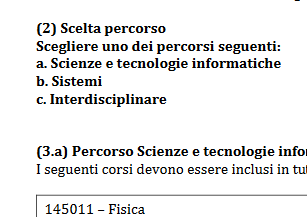
\includegraphics[width=0.8\textwidth, keepaspectratio]{curr-1.png}
					\end{figure}
					\vfill
					\begin{itemize}
						\item<7-> Scegliere il percorso di studi è un delirio
						\item<8-> Internet è il vostro migliore amico
					\end{itemize}
				\end{column}
				\visible<6->{
					\begin{column}{0.4\textwidth}
						\centering
						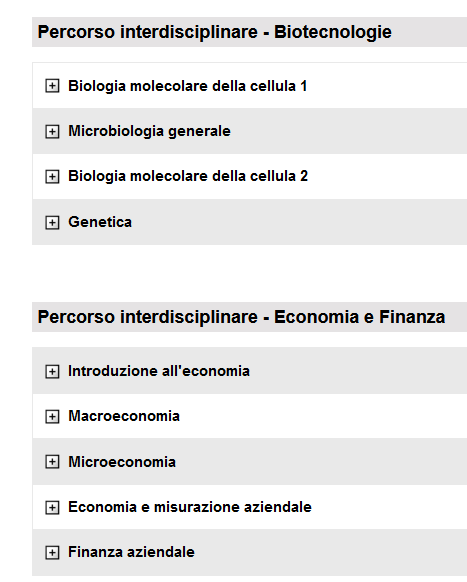
\includegraphics[width=0.8\textwidth, keepaspectratio]{curr-2.png}
					\end{column}	
				}
				\end{columns}
		}
	\end{frame}

	\begin{frame}{Ma c'è poca programmazione :(}
		\begin{itemize}
			\item<2-> I corsi incentrati sulla programmazione non sono molti
			\item<3-> la ragione è semplice: \emph{l'università non mira a insegnarvi a programmare}
			\item<4-> il motivo è sempre legato al discorso fatto prima
			\item<5-> avrete comunque modo di fare progetti e imparare molto
			\item<6-> ma se vi interessa solo quello, ci sono alternative mirate, meno costose e senza quegli sbatti che sono tipici di un percorso accademico e che potrebbero risultare pesanti se non ne avete interesse
			\begin{itemize}
				\item<7-> \url{https://www.tecnicosuperiorekennedy.it/}
				\item<7-> Corsi vari su Udemy e affini
			\end{itemize}
		\end{itemize}
	\end{frame}

	\begin{frame}{E la matematica?}
		Come avrete notato, di matematica (o affini) ce n'è:
			\begin{itemize}
				\item Analisi matematica I, 12 cfu
				\item Geometria e algebra lineare, 6 cfu
				\item Fondamenti matematici per l'informatica, 6 cfu
				\item Probabilità e statistica, 6, cfu
				\item Logica, 6 cfu
				\item Fisica, 6 cfu
			\end{itemize}
			\pause
			\vfill
			\huge{NO}
			\pause
			\Large{però in un certo senso} \huge{SÌ}
			\pause
			\Large{però comunque} \huge{NO}
			\pause
			\Large{gnnnn diciamo}\\ \centering\Huge{DIPENDE}
	\end{frame}

	\begin{frame}{Ma io \textit{$<$qualsiasi presunto requisito sentiate di non avere$>$}, avrò difficoltà?}
		Dove quei "presunti requisiti" potrebbero essere:
		\begin{itemize}
			\item apprezzare la matematica
			\item aver già programmato 
			\item incarnare lo stereotipo del nerd informatico boh idk
		\end{itemize}
		\pause
		\vfill
		\centering
		no.
	\end{frame}

	\section{Come si studia}
	\begin{frame}{Frequentare}
		\begin{itemize}
			\item<1-> Lezioni frontali tradizionali
			\item<2-> Esercitazioni\slash laboratori
			\item<3-> Sessioni di tutorato
			\item<4-> Condivisione materiale su Moodle o siti proprietari
			\item<5-> Comunicazione più giovane:
			\begin{itemize}
				\item Canale Telegram
				\item Server Discord
				\item Gruppi Slack
				\item Tanta roba
			\end{itemize}
		\end{itemize}
		\vfill
		\visible<6->{
			In periodo Covid-19:
			\begin{itemize}
				\item lezioni sincrone\slash asincrone, a discrezione dei docenti
				\item ci teniamo pure tutti i laboratori
				\item live più dirette, sessioni di Q \& A, insomma ci si parla
			\end{itemize}
		}
	\end{frame}

	\begin{frame}{Risorse}
		\begin{itemize}
			\item<1-> Internet
			\item<2-> Internet
			\item<3-> Internet
		\end{itemize}
		\vfill
		\visible<4->{
			Questo è valido in generale per tutta l'area STEM, ma soprattutto per informatica. \\
			Non solo: imparare a cercare, leggere, studiare (e anche scrivere) documentazione è parte integrante della formazione.
		}
		\vfill
		\visible<5->{
			Disclaimer importante: il \(95\%\) di tutto questo sarà fatto solo ed esclusivametne in \alert{inglese}.	
		}
	\end{frame}

	\begin{frame}{Autonomia}
		Occhio che questa cosa è molto molto molto molto molto molto molto importante.
		\begin{center}
			\begin{minipage}{\textwidth}
				\begin{alertblock}{Super tip per riuscire a imparare qualcosa}
					Fate in modo che vi importi.\\
					Fate le cose che vi vengono proposte.\\
					Fatele da soli e fatele assieme ad altri.\\
					Chiedetevi perché state facendo proprio così, chiedetevi cosa succederebbe se faceste diversamente.					
				\end{alertblock}
			\end{minipage}
		\end{center}
		\pause
		\scriptsize{ho finito con le lezioni di vita da boomer invecchiato male giuro}
	\end{frame}

	\section{Cosa si fa dopo}
	\begin{frame}{Tutti lavorano tranne me sad}
		\begin{columns}
			\begin{column}{0.4\textwidth}
				\begin{itemize}
					\item<1-> È vero che un laureato in informatica trova lavoro ez?
					\begin{itemize}
						\item<2-> Sì.
					\end{itemize}
					\item<3-> È vero che capita che lo trovi anche prima della laurea?
					\begin{itemize}
						\item<4-> Sì.
					\end{itemize}
					\item<5-> È vero che c'è molto interesse e mobilità anche nella ricerca?
					\begin{itemize}
						\item<6-> Sì.
					\end{itemize}
				\end{itemize}
			\end{column}
			\begin{column}{0.6\textwidth}
				\onslide<7>{
					inserire qui prova che è previsto  che lo studente abbia la possibilità di fare un'esprienza in ricerca
					% \centering
					% \includegraphics[width=0.5\textwidth, keepaspectratio, frame]{tirocinio.jpeg}	
				}
				\end{column}
		\end{columns}
	\end{frame}

	\section{Conclusione}
	\begin{frame}{Conclusione}
	Fioi domandate che altrimenti qua non si sa mai bene cosa sia meglio dire e cosa sia davvero utile
	\vfill
	contatti	
	\end{frame}

\end{document}